\documentclass[dvipdfm]{article}
\usepackage[dvips]{graphicx}
\usepackage[usenames,dvipsnames]{color}
\usepackage[dvipdfm]{hyperref}
\title{\color{blue}Latex Support Test File}
\author{\color{green}Mark A. Wicks}
\begin{document}
\maketitle
\section{Introduction}
This document is primarily intended
to test the functionality
of some \LaTeX\space packages that require
driver support for their functionality.
It is quick-and-dirty.
It is not intended to be pretty, and
does not demonstrate good ways to use these packages
(In fact, it demonstrates some bad ways to use these packages).

This is a \href{http://odo.kettering.edu/dvipdfm/}{test too see how
well dvipdfm handles links that need to be broken over several lines.  This
will only work if you have dvipdfm version 0.12.4 or later
and have installed {\tt hdvpdfm.def} from the version 0.12.4 or
later distribution.}

\section{LaTeX Support Information}
Dvipdfm support for the hyperref \LaTeX\space package is 
in hyperref versions 6.44 (12/07/98) and above, available on CTAN.
Dvipdfm is now supported in the
standard \LaTeX\space release (via the ``color'' and ``graphics'' packages) in
\LaTeX\space releases dated later than December 1998.

If you have an older LaTeX\space and don't want to upgrade,
this distribution of {\tt dvipdfm} includes
the {\tt .def} files required to support
the
{\textcolor{green}{c}%
\textcolor{red}{o}%
\textcolor{blue}{l}%
\textcolor{green}{o}%
\textcolor{red}{r}
and
\scalebox{1.3}[1]{\rotatebox{15}{gr%
  \scalebox{1.3}[1]{\rotatebox{15}{ap%
    \scalebox{1.3}[1]{\rotatebox{15}{hi%
       \scalebox{1.3}[1]{\rotatebox{15}{cs}}}}}}}}
packages.}
You may also need to modify {\tt color.sty}, {\tt graphics.sty},
and {\tt hyperref.sty} so that they
recognize {\tt dvipdfm} as a driver.
Once these {\tt .def} files are installed,
you should be able to use {\tt dvipdfm}
with \LaTeX\space for many applications.

After running \LaTeX\space on this
document, {\tt hyperref}
should produce a hyperlinked
document, complete with an outline.

\newpage
\section{Graphics Support}
Currently, JPEG and PDF image
inclusion are supported.

\subsection{JPEG Image Inclusion}
Figure~\ref{fig:author}
shows a photograph of the author
that was obtained from a JPEG file.
A small file with the extension of {\tt .bb}
supplies the bounding box to the \LaTeX\space
Graphics package.  For PDF and JPEG files,
this bounding box can easily be created by running
the {\tt ebb} utility included with this
distribution of {\tt dvipdfm}.

\begin{figure}
  \begin{center}
    
\includegraphics{mwicks.jpeg}
  \end{center}

  \caption{A photograph of the author.}
  \label{fig:author}
\end{figure}

\subsection{PDF Image Inclusion}
Figure~\ref{fig:circuit} shows
an electronics circuit,
drawn with XFig, distilled,
and then included as PDF file.
It has been mangled for testing purposes.
\begin{figure}
  \begin{center}
     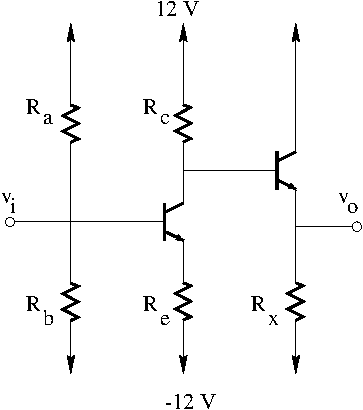
\includegraphics[viewport=30 30 150 150,angle=20,width=2.0in,height=3.0in]{transistor}
  \end{center}

  \caption{A simple two-stage transistor circuit (mangled by includegraphics
options).}
  \label{fig:circuit}
\end{figure}

\begin{figure}
  \begin{center}
    
\includegraphics[clip,angle=20,height=1.0in,width=2.0in]{something.eps}
  \end{center}

  \caption{A second included figure}
  \label{fig:something}
\end{figure}

\end{document}
